\documentclass[aspectratio=169,11pt]{beamer}

\usetheme{default}
\usepackage[T1]{fontenc}
\usepackage{lmodern}
\usepackage{booktabs}
\usepackage{tikz}
\usepackage{pgfplots}
\pgfplotsset{compat=1.17}
\usetikzlibrary{shapes.geometric,positioning,arrows.meta}

% ---- palette: black box -> white box, amber = illumination ----
\definecolor{inkDark}{HTML}{141414}
\definecolor{inkCard}{HTML}{1F1F1F}
\definecolor{paperLight}{HTML}{F5F5F5}
\definecolor{ink}{HTML}{1A1A1A}
\definecolor{mute}{HTML}{6B6B6B}
\definecolor{accent}{HTML}{E8A33D}
\definecolor{accentDk}{HTML}{B87D1E}
\definecolor{lineGrey}{HTML}{E2E2E2}

\setbeamercolor{background canvas}{bg=white}
\setbeamercolor{normal text}{fg=ink}
\setbeamercolor{title}{fg=white}
\setbeamercolor{frametitle}{fg=ink,bg=white}
\setbeamercolor{structure}{fg=accentDk}
\setbeamercolor{block title}{fg=white,bg=inkDark}
\setbeamercolor{block body}{fg=ink,bg=paperLight}
\setbeamercolor{itemize item}{fg=accentDk}
\setbeamerfont{frametitle}{series=\bfseries,size=\Large}
\setbeamertemplate{navigation symbols}{}
\setbeamertemplate{itemize item}{\textbullet}
\setbeamertemplate{footline}{%
  \hfill\usebeamercolor[fg]{mute}{\color{mute}\scriptsize\insertframenumber\,/\,\inserttotalframenumber}\hspace{3mm}\vspace{2mm}
}

\newcommand{\kicker}[1]{{\scriptsize\bfseries\color{accentDk}\MakeUppercase{#1}}\\[2pt]}

\title{From Black Box to White Box}
\subtitle{A Case Study in Autoresearch}
\author{Christian Block \\ \small Research project with Prof.\ Ramesh}
\date{July 2026}

\begin{document}

% ================= Title =================
{
\setbeamercolor{background canvas}{bg=inkDark}
\begin{frame}[plain]
\vspace{4mm}
{\scriptsize\bfseries\color{accent}\MakeUppercase{A case study in autoresearch}}\\[10pt]
{\Huge\bfseries\color{white} From Black Box \color{mute!40!white}to White Box}\\[10pt]
{\large\color{white!80!black} Measuring how an instruction file shapes an autonomous research agent's behavior}\\[18pt]
{\color{accent}\rule{2.2cm}{1pt}}\\[10pt]
{\bfseries\color{white} Christian Block}\\
{\small\color{white!60!black} Research project with Prof.\ Ramesh \quad$\bullet$\quad July 2026}
\end{frame}
}

% ================= Motivation =================
\begin{frame}{Motivation}
\kicker{Why this matters}
\small\textbf{An autoresearch loop is a language model running its own research cycle:} read instructions, propose an experiment, run it, interpret, decide what's next --- repeating without a person in the loop.
\vspace{2.5mm}

\begin{columns}[T,onlytextwidth]
\column{0.48\textwidth}
\begin{block}{\small What we observe}
\footnotesize
Change the instruction file --- \texttt{program.md} --- and the agent's research \emph{process} changes: how many experiments it runs, how broadly it searches, how it stops.
\end{block}
\column{0.48\textwidth}
\begin{block}{\small What we don't know}
\footnotesize
Which specific sentence caused which specific change, and by how much. The relationship is observed, never explained.
\end{block}
\end{columns}
\vspace{1.5mm}

\begin{block}{\small Why that gap is costly}
\footnotesize
Without it we cannot \textbf{predict} behavior under an untried instruction, and we cannot \textbf{explain} behavior to someone else in a way they can act on. ``It behaved differently because I changed the instructions'' is not actionable; ``it ran fewer experiments because the stopping rule was stricter, which explains half the variation'' is.
\end{block}
\end{frame}

% ================= The approach =================
\begin{frame}{The approach: borrow from AutoML}
\kicker{Same problem, already solved once}
AutoML already has tools for exactly this kind of question --- just applied to hyperparameters instead of instructions. An instruction file is, structurally, no different: a set of discrete, largely independent choices that jointly determine behavior.
\vspace{4mm}

\begin{columns}[T,onlytextwidth]
\column{0.32\textwidth}
\begin{block}{\centering 1}
\centering\small
\textbf{Ablation design}\\[4pt]
\raggedright A small, principled subset of configurations to run --- not all of them, not random ones.
\end{block}
\column{0.32\textwidth}
\begin{block}{\centering 2}
\centering\small
\textbf{Surrogate model}\\[4pt]
\raggedright An interpretable model: which axis explains how much of the behavior.
\end{block}
\column{0.32\textwidth}
\begin{block}{\centering 3}
\centering\small
\textbf{Causal validation}\\[4pt]
\raggedright Predict a held-out configuration's behavior, then check it for real.
\end{block}
\end{columns}
\end{frame}

% ================= Configuration space =================
\begin{frame}{Step 2 --- five instructional axes}
\kicker{Turning program.md into a configuration vector}
\small
Every possible \texttt{program.md} is generated from a 5-bit vector; a template guarantees two files differ only in the axes intentionally varied.
\vspace{3mm}

\begin{tabular}{@{}p{1.1cm}p{2.0cm}p{8.6cm}@{}}
\toprule
\textbf{Axis} & \textbf{Name} & \textbf{Two levels} \\
\midrule
M & Metric & Vague (``judge appropriate'') vs.\ precise (CV accuracy + std) \\
B & Breadth & Stay in one model family vs.\ free to compare both \\
S & Stopping & Fixed budget of 3 vs.\ adaptive, up to 8 \\
O & Output & Terse and numeric vs.\ fully reasoned prose \\
E & Emphasis & Explore broadly first vs.\ refine immediately \\
\bottomrule
\end{tabular}
\end{frame}

% ================= Real experiments =================
\begin{frame}{Step 3 --- real experiments, not simulated ones}
\kicker{Design and execution}
\begin{columns}[T,onlytextwidth]
\column{0.56\textwidth}
\small
A resolution-III \textbf{Plackett--Burman design} selects 8 of the 32 possible configurations --- enough to estimate every axis's individual effect without bias.

\vspace{3mm}
Every configuration runs against a real scikit-learn task: tune Random Forest / Gradient Boosting on the Breast Cancer Wisconsin dataset. Every number the agent sees is a genuine measurement, never invented.

\column{0.4\textwidth}
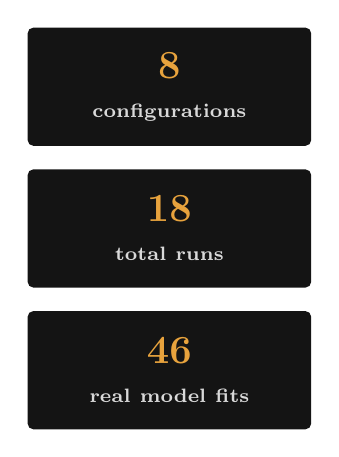
\begin{tikzpicture}
\foreach \v/\l/\i in {8/configurations/0, 18/total runs/1, 46/real model fits/2} {
  \node[fill=inkDark, rounded corners=2pt, minimum width=3.6cm, minimum height=1.5cm, text width=3.2cm, align=center] at (0,-1.8*\i) {
    \color{accent}\Large\bfseries \v \\[2pt] \color{white!85!black}\scriptsize \l
  };
}
\end{tikzpicture}
\end{columns}
\end{frame}

% ================= Behavioral encoding =================
\begin{frame}{Step 4 --- six numbers per run}
\kicker{Each answers a specific question}
\begin{columns}[T,onlytextwidth]
\column{0.32\textwidth}
\begin{block}{\small How much research happened}
\footnotesize
\begin{itemize}
\item \# experiments run
\item \# model families tried
\item search width (hyperparameter spread)
\end{itemize}
\end{block}
\column{0.32\textwidth}
\begin{block}{\small Did it pay off}
\footnotesize
\begin{itemize}
\item best cross-validated accuracy reached
\end{itemize}
\end{block}
\column{0.32\textwidth}
\begin{block}{\small Can the pipeline be trusted}
\footnotesize
\begin{itemize}
\item verbosity (known ground-truth check)
\item distance to a reference research trace
\end{itemize}
\end{block}
\end{columns}
\end{frame}

% ================= Results: surrogate model =================
\begin{frame}{Step 5 --- which axis explains which behavior}
\kicker{Surrogate model results}
\begin{columns}[T,onlytextwidth]
\column{0.56\textwidth}
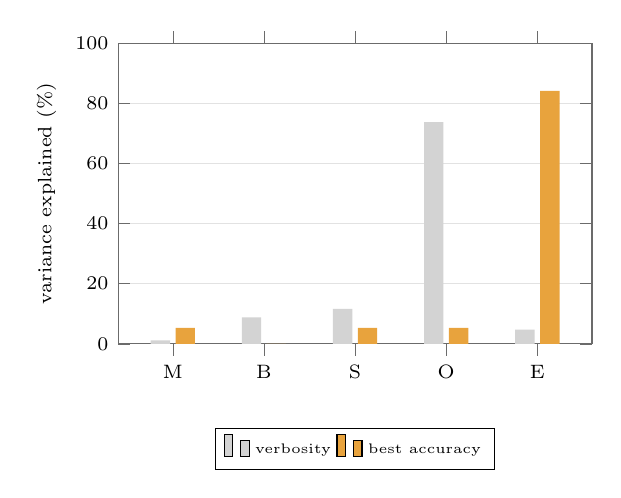
\begin{tikzpicture}
\begin{axis}[
  ybar, bar width=7pt, width=7.6cm, height=5.4cm,
  ymin=0, ymax=100, ylabel={\scriptsize variance explained (\%)},
  symbolic x coords={M,B,S,O,E}, xtick=data,
  tick label style={font=\scriptsize}, ylabel style={font=\scriptsize},
  enlarge x limits=0.15,
  legend style={font=\tiny, at={(0.5,-0.28)}, anchor=north, legend columns=2},
  ymajorgrids, grid style={lineGrey, line width=0.3pt},
  axis line style={mute}, tick style={mute},
]
\addplot[fill=lineGrey!150!white, draw=none] coordinates {(M,1.1) (B,8.8) (S,11.6) (O,73.7) (E,4.7)};
\addplot[fill=accent, draw=none] coordinates {(M,5.3) (B,0.0) (S,5.3) (O,5.3) (E,84.1)};
\legend{verbosity, best accuracy}
\end{axis}
\end{tikzpicture}
\column{0.4\textwidth}
\begin{block}{\small Output format $\rightarrow$ verbosity}
\footnotesize 74\% of variance, $p=0.027$. Expected --- confirms the pipeline works end to end.
\end{block}
\vspace{2mm}
\begin{block}{\small Emphasis $\rightarrow$ accuracy}
\footnotesize 84\% of variance. Refine-immediately beats explore-first by $\sim$0.25 accuracy points --- a non-obvious effect.
\end{block}
\end{columns}
\end{frame}

% ================= Causal validation =================
\begin{frame}{Step 6 --- predict first, then run it for real}
\kicker{Causal validation}
\small One configuration was held out of the design; its prediction was written down before it was ever executed.
\vspace{3mm}

\begin{columns}[T,onlytextwidth]
\column{0.48\textwidth}
\begin{block}{Number of experiments}
\begin{tabular}{@{}p{2.6cm}p{2.6cm}@{}}
{\scriptsize\color{mute} PREDICTED}\newline{\Large\bfseries\color{mute} 3.25} &
{\scriptsize\color{accentDk} OBSERVED}\newline{\Large\bfseries 3.00}
\end{tabular}\\[4pt]
{\scriptsize\itshape Off by a quarter of an experiment --- essentially exact.}
\end{block}
\column{0.48\textwidth}
\begin{block}{Best accuracy reached}
\begin{tabular}{@{}p{2.6cm}p{2.6cm}@{}}
{\scriptsize\color{mute} PREDICTED}\newline{\Large\bfseries\color{mute} 0.9648} &
{\scriptsize\color{accentDk} OBSERVED}\newline{\Large\bfseries 0.9610}
\end{tabular}\\[4pt]
{\scriptsize\itshape Off by $\sim$0.004 --- small, explainable miss.}
\end{block}
\end{columns}
\vspace{4mm}

\begin{block}{}
\small\color{white}
\textbf{\color{accent}A wrong-but-explainable prediction} is more useful than a validation step that's skipped, or one that always happens to be right --- it points straight at what the design couldn't see: an interaction between axes.
\end{block}
\end{frame}
{\setbeamercolor{block body}{bg=inkDark,fg=white}}

% ================= Black box to white box =================
{
\setbeamercolor{background canvas}{bg=inkDark}
\setbeamercolor{normal text}{fg=white}
\setbeamercolor{frametitle}{fg=white,bg=inkDark}
\begin{frame}{A white box --- of behavior, not of mechanism}
\kicker{How much of the black box actually opened}
\begin{columns}[T,onlytextwidth]
\column{0.48\textwidth}
{\bfseries\color{accent} What became visible}
\footnotesize
\begin{itemize}
\item \texttt{program.md} became a labeled 5-axis vector, not an opaque file
\item The axis $\to$ behavior link is a readable linear model, not another black box
\item One prediction was checked against a real run before the outcome was known
\end{itemize}
\column{0.48\textwidth}
{\bfseries\color{mute!60!white} What stayed opaque}
\footnotesize
\begin{itemize}
\item Nothing here explains the model's internal mechanism --- weights, attention, computation
\item Findings describe this study's own small system, not autoresearch loops in general
\item Only the \emph{method} is a candidate for generalizing --- not yet the specific numbers
\end{itemize}
\end{columns}
\end{frame}
}

% ================= Limitations =================
\begin{frame}{Limitations, stated plainly}
\kicker{Read the results with these firmly in mind}
\small
\begin{columns}[T,onlytextwidth]
\column{0.48\textwidth}
\begin{block}{\footnotesize 1. Agent = the author}
\footnotesize Every run's decisions were made by someone who already knew this was an ablation study --- a real confound.
\end{block}
\vspace{2mm}
\begin{block}{\footnotesize 2. Human trace is authored}
\footnotesize Real experiment numbers, but an invented reasoning process --- not an observed human.
\end{block}
\column{0.48\textwidth}
\begin{block}{\footnotesize 3. Small sample}
\footnotesize 2 repeats/config; 8 configs $\to$ only 2 residual degrees of freedom in every model.
\end{block}
\vspace{2mm}
\begin{block}{\footnotesize 4. Narrow scope}
\footnotesize One dataset, two model families, five axes --- generalization not yet shown.
\end{block}
\end{columns}
\end{frame}

% ================= Conclusion =================
{
\setbeamercolor{background canvas}{bg=inkDark}
\setbeamercolor{normal text}{fg=white}
\setbeamercolor{frametitle}{fg=white,bg=inkDark}
\begin{frame}{A method, demonstrated end to end}
\kicker{Conclusion \& next steps}
\small
Every step ran against real, executed machine-learning experiments --- configuration space, ablation design, surrogate model, and a causal check that made a falsifiable prediction and tested it.
\vspace{4mm}

\begin{enumerate}
\small
\item Replace the author-as-agent substitution with independent, fresh-context model calls
\item Record an actual human reference session to replace the authored trace
\item Expand the design (resolution IV+) to estimate the interaction Step 6 flagged
\item Repeat across more than one dataset to test generality
\end{enumerate}

\vspace{6mm}
{\scriptsize\color{mute!70!white} Full report: github.com/topoftheblock/autoresearch}
\end{frame}
}

\end{document}
